\subsection{Discretización de ecuaciones en espacio de estado}

Sea el sistema
\[(1)
    \left\{
        \begin{array}{lll}
            \dot{x}(t) = Ax(t) + Bu(t) \\
            y(t) = Cx(t)
        \end{array}
    \right.
\]
con condición inicial \( x(0) = x_{0} \)

El problema de discretización consiste en obtener un sistema dinámico equivalente para el sistema (1) en tiempo discreto de la forma
\[
    \left\{
        \begin{array}{lll}
            \dot{x}(k+1) = Ax(k) + Bu(k) \\
            y(k) = Cx(k)
        \end{array}
    \right.
\]

donde
\[
    \left\{
        \begin{array}{lll}
            \dot{x}((k+1)T) = Ax(kT) + Bu(kT) \\
            y(kT) = Cx(kT)
        \end{array}
    \right.
\]

\begin{figure}[ht]
    \centering
        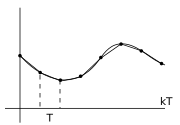
\includegraphics[scale=0.30]{Control de Sistemas Mecatronicos Figuras/20 Continuo a Discreto.png}
        \caption{Continuo a discreto}
\end{figure}

La solución de la ecuación (1) es 
\[
    (2) \;\; x(t) = e^{At}x(0) + \int_{0}^{t}e^{ A(t-\tau) }Bu(\tau)d\tau
\]

Haciendo \( t = (k+1)T \) en la ecuación (2)
\[
    (3) \;\; x((k+1)T) = e^{ A(k+1)T }x(0) + e^{ A(k+1)T } \int_{0}^{ (k+1)T } e^{ -A\tau }Bu(\tau)d\tau
\]

Haciendo \( t = kT \) en la ecuación (2)
\[
    (4) \;\; x(kT) = e^{ AkT }x(0) + e^{ AkT }\int_{0}^{kT} e^{ -A\tau }Bu(\tau)d\tau
\]

Multiplicar (4) por \( e^{AT} \)
\[
    \begin{split}
        (5) \;\; e^{ AT }x(kT) & = e^{ AT }e^{AkT}x(0) + e^{ AT }e^{AkT}\int_{0}^{kT} e^{ -A\tau }Bu(\tau)d\tau \\
        & = e^{A(k+1)T}x(0) + e^{A(k+1)T}\int_{0}^{kT} e^{-A\tau}Bu(\tau)d\tau
    \end{split}
\]

Restarle (5) a (3)
\[
    \begin{split}
        x((k+1)T) - e^{AT}x(kT) & = e^{A(k+1)T} \int_{0}^{(k+1)T} e^{-A \tau}Bu(\tau)d\tau - \\ 
        & e^{A(k+1)T}\int_{0}^{kT}e^{-A \tau}Bu(\tau)d\tau \\
        & = e^{A(k+1)T}\int_{kT}^{(k+1)T}e^{-A \tau}Bu(\tau)d\tau \\
        x((k+1)T) & = e^{AT}x(kT) + e^{A(k+1)T}\int_{kT}^{(k+1)T}e^{-A \tau}Bu(\tau)d\tau 
    \end{split}
\]

Se asume \( u(t) \) es constante para \( kT \leq t \leq (k+1)T \)
\[
    \begin{split}
        (6) \;\; x((k+1)T) & = e^{AT}x(kT) + e^{A(k+1)T}\int_{kT}^{(k+1)T}e^{-A \tau}d\tau Bu(kT)  
    \end{split}
\]

Se puede ver que \( e^{A(k+1)T} \int_{kT}^{(k+1)T} e^{-A\tau} d\tau \) se puede resolver por cambio de variable 
\[
    \begin{split}
        u & = -A\tau \\
        du & = -Ad\tau \\
        -A^{-1}du & = d\tau \\
        \text{con limites} \\
        u_{kT} & = -AkT \\
        u_{(k+1)T} & = -A(k+1)T
    \end{split}
\]
\[
    \begin{split}
        e^{A(k+1)T} \int_{kT}^{(k+1)T} e^{-A\tau} d\tau & = e^{A(k+1)T} \int_{-AkT}^{-A(k+1)T} e^{u}(-A^{-1})du \\
        & = e^{A(k+1)T} \big|_{-AkT}^{-A(k+1)T} e^{u}(-A^{-1}) \\
        & = e^{A(k+1)T} [e^{-A(k+1)T} - e^{-AkT}] (-A^{-1}) \\
        & = [e^{0} - e^{AT}](-A^{-1}) \\
        & = [e^{AT} - I]A^{-1}
    \end{split}
\]

El resultado es el mismo si se aplica la integral por un periodo \( T \), usando el mismo cambio de variable, pero cambiando los limites a 
\[
    \begin{split}
        u_{T} & = -AT \\
        u_{0} & = 0
    \end{split}
\]
\[
    \begin{split}
        e^{ AT } \int_{0}^{T} e^{ -A\tau } d\tau & = e^{ AT } \int_{0}^{ -AT } e^{ u }(-A^{-1})du \\
        & = e^{ AT } \big|_{0}^{-AT} e^{u}(-A^{-1}) \\
        & = e^{ AT } [ e^{-AT} - e^{0} ] (-A^{-1}) \\
        & = [ e^{0} - e^{AT} ](-A^{-1}) \\
        & = [ e^{ AT } - I ]A^{-1}
    \end{split}
\]

por lo tanto, es posible sustituir la integral de (6)
\[
    \begin{split}
        (6) \;\; x((k+1)T) & = e^{ AT }x(kT) + e^{ AT } \int_{0}^{T} e^{ -A\tau } d\tau Bu(kT) \\
        & = e^{ AT }x(kT) + \int_{0}^{T} e^{ A(T-\tau) } d\tau Bu(kT)
    \end{split}
\]

se realiza un cambio de variable 
\[ 
    \begin{split}
        \lambda & = T - \tau \\
        d\lambda & = -d\tau \\
        \text{con limites} \\
        \lambda_{T} & = 0 \\
        \lambda_{0} & = T
    \end{split} 
\]
\[
    \begin{split}
        \;\; x((k+1)T) & = e^{ AT }x(kT) - \int_{T}^{0} e^{A\lambda} d\lambda Bu(kT) \\
        & = e^{ AT }x(kT) + \int_{0}^{T} e^{ A\lambda } d\lambda Bu(kT)
    \end{split}
\]

Entonces se definen
\[
    \begin{split}
        A(t) & = e^{ AT } \\
        B(t) & = \big( \int_{0}^{T} e^{ A\lambda } d\lambda \big) B
    \end{split}
\]